\documentclass[norsk,a4paper,12pt]{article}
\usepackage[T1]{fontenc} %for å bruke æøå
\usepackage[utf8]{inputenc}
\usepackage{graphicx} %for å inkludere grafikk
\usepackage{verbatim} %for å inkludere filer med tegn LaTeX ikke liker
\usepackage{amsfonts}
%\usepackage[framed]{mcode} %for å få inn matlabkode
\usepackage{listings}
\usepackage[margin=1.2cm]{caption} % skalere figur text
\usepackage{subfigure}

\bibliographystyle{plain}
\usepackage{parskip}
\usepackage{babel, textcomp, color, amsmath, amssymb, tikz, subfig, float}
\renewcommand{\captionfont}{\sffamily\small} 
\renewcommand{\captionlabelfont}{\bf} 
\fboxsep=0mm % ramme inn bilder


\title{FYS3150 - Project 3}
\author{Steffen Brask}
\date{\today}


\begin{document}

\maketitle

\begin{center}
GIT link: https://github.com/steffemb/project3/tree/master/project3/solarsystem
\end{center}


\newpage


\section*{Abstract}

In this project we are going to model the solar system. The goal is not actually to model the solar system but rather to
make an outline of a system which can be improved upon later. And then test the numerical stability.

Much of the work in this project is purely programming, and structuring a class hierarchy so it is as moldable as possible.

We will see that for large systems Runge Kutta methods is the best way to solve the ODE's, everything else gives numerical errors
that are unacceptable, unless you use a very small step length, so small that it gets hard to compute. In fact for complicated systems like the
whole solar system we should use something better than even Runge Kutta 4, like adaptive methods. 


\section*{Introduction}

Solving ordinary differential equations is not new science. It is something we have done with pen and paper, but also something
we have programmed in many courses earlier. So what is new in this project? To be honest not that much, at least not on the ODE
solver part. What is new is the object orientation, which is important when modeling such a big system. If I where to model
the solar system in a python script it would probably get very messy fast. Not to talk about what a nightmare it would have been 
to add new objects to the system.

So i guess thats our motivation for this project. We will take a closer look at Runge Kutta 4 also. And of course, we can brag about
it too our friends.

\section*{Solution}

In this project i opted  to use the class structure given at the computer lab. Details can be found at 
the github link given on the front page. 

First i want to do a short rundown of how the structure works. On top we have a class ``Solarsystem''. Inside ``Solarsystem''
we have objects called ``CelestialBody''. Each Body in the solar system gets it's own object reference. For example 
in the Earth-Sun system Earth would be ``mySolarsystem.objects[1]''. And this object contains all the information about
Earth in form of 3 dim. vectors or double float numbers. The ``Solarsystem'' only contains information at a specific time t. By using 
the ``Integrate'' class we update all the information in the ``Solarsystem'' from t to (t + dt), where dt is the step length.
So sending a solar system to the integrate class will only update the solar system one step. ``Solarsystem'' also contains a 
couple of other functions, mostly self explanatory, but the most important is ``void Force()'' which gives every object in a ``Solarsystem''
a force vector which is the sum of all acting forces and also updates kinetic and potential energy for the object.

One of the main tasks in this project is to program the ``Force()'' function. To do this we start with Newtons gravitational 
force between two objects, 

\begin{align}
 F = G\frac{mM}{r^2}, or, \vec{F} = G\frac{mM}{r^3} \vec{r},
\end{align}

Where m and M are the masses, and G is the gravitational constant. First we need to decompose the force to $F_x$, $F_y$ and $F_z$.
scince $\vec{r} = {r_x, r_y, r_z}$ we get, 

\begin{align}
 \vec{F_x} = G\frac{mM}{r^3} \vec{r_x},  \vec{F_y} = G\frac{mM}{r^3} \vec{r_y},  \vec{F_z} = G\frac{mM}{r^3} \vec{r_z},
\end{align}

If we now have an n-body system we will need to sum n-1 of these forces for each body to find the total force acting on each body.
we will fix the origin of the system in space, and we then get the $\vec{r_i}$ vector easily by taking $\vec{r_{\text{ObjectOfInterest}}} - \vec{r_{\text{OtherObject}}}$.
And the total force on an object is, 

\begin{align}
 \sum_{i = 1}^{i = n-1}\vec{F_i} = G\frac{ M_{ObjectOfInterest} M_{Object_i} } {r^3} \vec{r_i}.
\end{align}

Now that we have our forces in x, y, z our last task before we have a working simulation is to solve the equations

\begin{equation}
 \frac{d^2 x}{dt^2} = \frac{\sum F_x}{M_{Object}}, 
\end{equation}

\begin{equation}
 \frac{d^2 y}{dt^2} = \frac{\sum F_y}{M_{Object}}, 
\end{equation}

\begin{equation}
 \frac{d^2 z}{dt^2} = \frac{\sum F_z}{M_{Object}}, 
\end{equation}


for every object in the system.



\subsection*{Runge Kutta 4 method}

The main method for solving the ODE's in this project is the forth order Runge Kutta method. We will prefer using this method 
since it gives us a truncation error of $o(h^4)$ apposed to $o(h^3)$ for Verlet method or $o(h^2)$ for Euler'r method.

Mathematically the Runge Kutta method goes as follows:

First we need

\begin{align}
 k_1 = f(t_i, y_i)dt,
\end{align}

I have called the step $dt$ here, it is customary to write $h$ instead of $dt$, but in our case our step is in time, so i called
it $dt$. $k_1$ is nothing but Eulers method, that is, it is the slope at $t_i, y_i$. In our case the function $f$ is the force divided
by the mass of the object. second we need

\begin{align}
 k_2 = f(t_i + dt/2, y_i + k_{1}/2)dt.
\end{align}

$k_2$ is a prediction of the slope at the midpoint. In our case we therefore need to calculate the forces on the objects at $t + dt/2$
using $k_1$ as a prediction. Third we need 

\begin{align}
 k_3 = f(t_i + dt/2, y_i + k_{2}/2)dt.
\end{align}

With $k_3$ we do the same except we say that $k_2$ is a new and ``better'' prediction therefore we use that instead of $k_1$.
The forth step is

\begin{align}
 k_4 = f(t_i + dt, y_i + k_3)dt,
\end{align}

this is to predict the slope at $y_{i+1}$ at $t_i + dt$. We now have everything we need for our final prediction

\begin{align}
 y_{i+1} = y_i + \frac{1}{6} [k_1 + 2k_2 + 2k_3 + k_4].
\end{align}

What we already have is the right hand side of eq 4, 5, 6. Which means we already have the acceleration of the objects at time $t$.
so when we calculate $y_{i+1}$ this will be the velocity in x, y, z. And then we can just run the algorithm again to get the positions.

\begin{figure}[H]
  \begin{center}
    \subfigure[Runge Kutta 4]{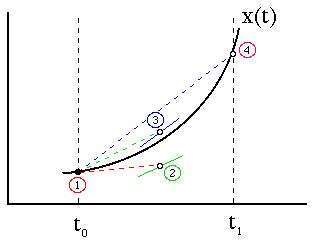
\includegraphics[scale=0.5]{rk4.jpeg}}
  \end{center}
 \caption{\textit{Figure for illustrating rk4 method graphically. 1, 2, 3, 4 stands for k1, k2, k3, k4. }}
  \label{fig:edge}
\end{figure}

One problem in the class hierarchy is that we only have one given vector for velocity, position etc and by updating them with, say, $k_2$
the object ``forgets'' about $k_1$. So to solve this i had to make four copy solar systems and compute $k_1, k_2, k_3, k_4$ in 
one copy each. This makes for a messy and long code, and is therefore something i would try to improve for the future.

\subsection*{Setting up the solar system}

When setting up the solar system we need to give it a center of mass so that everything keeps its symmetry. In an n-body system
the center of mass is given by

\begin{align}
 R = \frac{1}{M} \sum_{i=1}^{n} m_i r_i
\end{align}

where $M$ is the sum of the masses of all the objects. We will start with the Sun-Earth-Jupiter system.

We also need initial values for all the objects. Since we are in dimensions AU and years we can give the Earth x position $1-CenterOfMass$,
and velocity $2*\pi$. This is not exactly correct, in reality the Earth has a slightly elliptical orbit. For Jupiter and the Sun it 
is slightly more difficult. The positions are easy, they are $position-CenterOfMass$, that is $0-CenterOfMas$ for the Sun, and $5.2-CenterOfMas$
for Jupiter. For the velocities we can use the formula for centripetal acceleration

\begin{align}
 a = \frac{v^2}{r} = \frac{F}{m} \Rightarrow v = \sqrt{r\frac{F}{m}}
\end{align}

So with the positions given over we now know the magnitude of v. So to make this simple we place all objects along the x-axis and give them velocities
in the y-axis. We give the sun negative values and everything else positive. This is because the center of mass will be between 
the Sun and everything else. If we did not give the Sun and everything else opposite velocity directions they would not orbit the 
origin where we wish the center of mass to be.

To check  if we are doing things right we can compute the potential energy, the kinetic energy, and the angular momentum. 
in the case that we have circular orbits these should all be constants, on each object, but also the total. This is because 
it is always a balance between kinetic and potential energy. When the orbit is circular the magnitude of $\vec{r}$ is a constant, which
makes all the latter constants. If we want to play with elliptical orbits, as a test, we can check the total energy, which should 
always be conserved.

\section*{Results}

The first result we get is that for the case where we make circular orbits the energy is indeed conserved, we can also see from a 
plot that the system is doing something that is intuitive pleasing.

\begin{figure}[H]
  \begin{center}
    \subfigure[Sun Earth Jupiter after 0,75y]{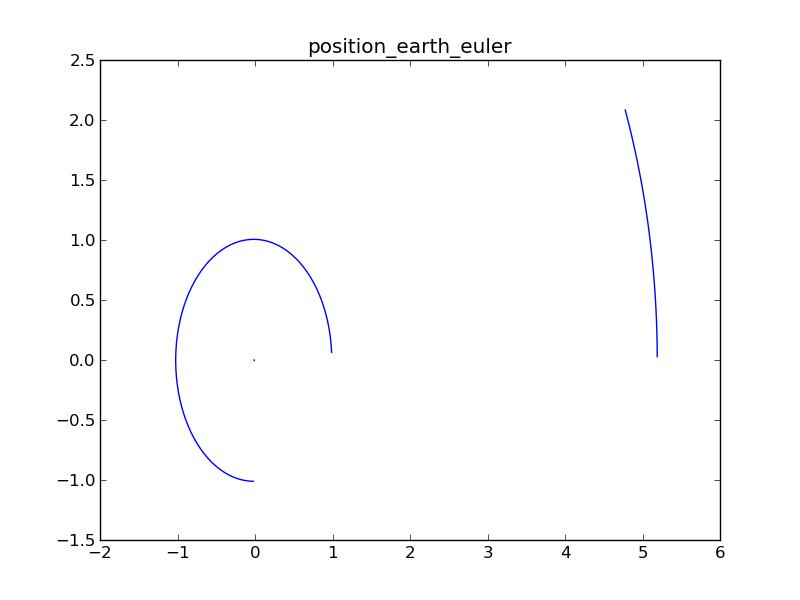
\includegraphics[scale=0.2]{sun_earth_jupiter_075y.jpg}}
    \subfigure[Sun Earth Jupiter after 10y]{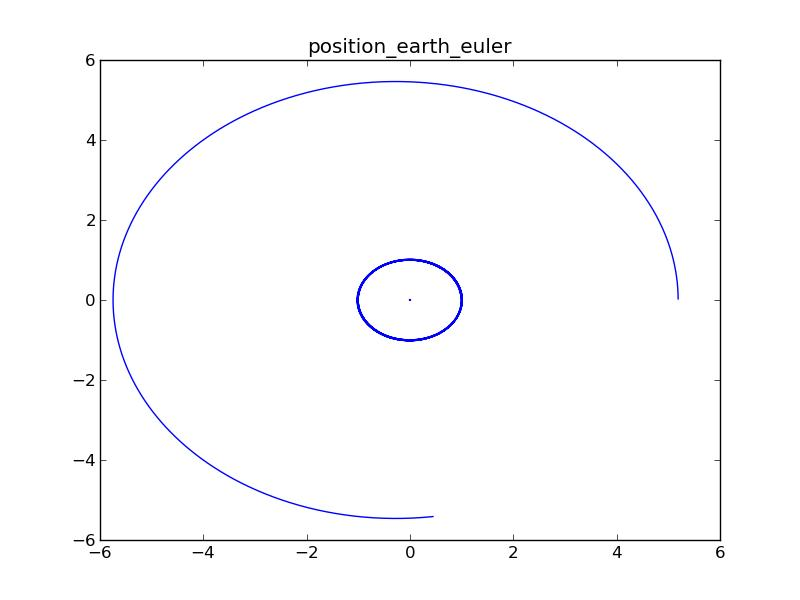
\includegraphics[scale=0.2]{sun_earth_jupiter_10y.jpg}}
  \end{center}
 \caption{\textit{ }}
  \label{fig:edge}
\end{figure}

If we test for different values of dt and plot we see that not all values gives us something that works. 

\begin{figure}[H]
  \begin{center}
    \subfigure[stability at dt = 0,5]{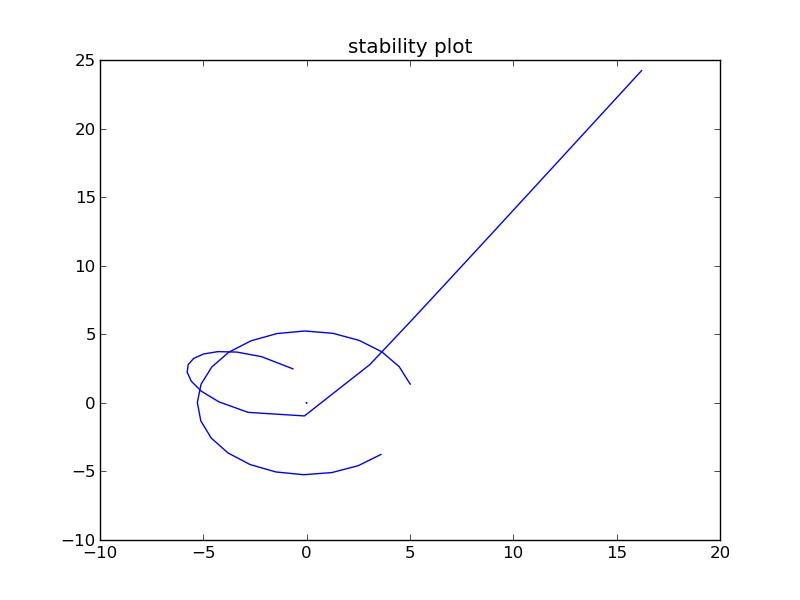
\includegraphics[scale=0.2]{unstable_dt_0,5.jpg}}
    \subfigure[stability at dt = 0,7]{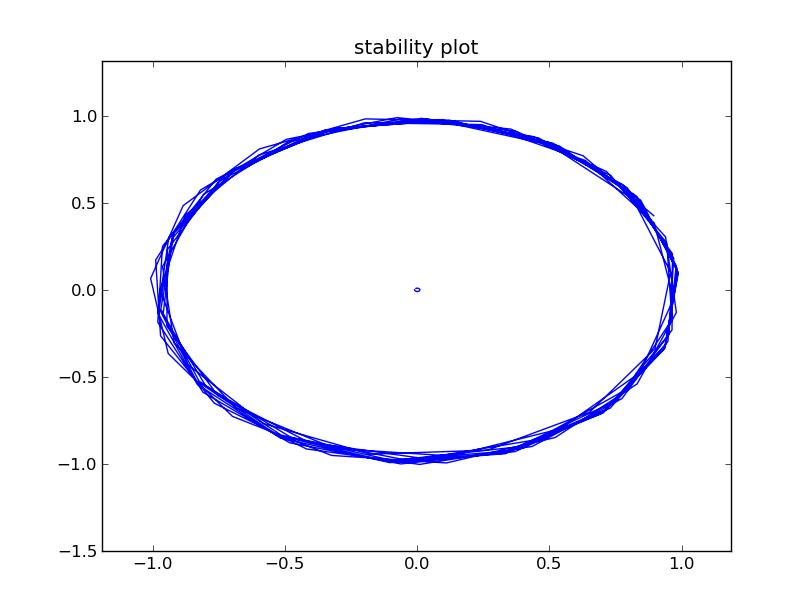
\includegraphics[scale=0.2]{unstable_dt_0,7.jpg}}
  \end{center}
 \caption{\textit{ }}
  \label{fig:edge}
\end{figure}

For dt = 0,5 we see that something really strange is happening. Although the total energy is conserved this is not physically 
pleasing. When testing for dt = 0,7 we see that we have a stable orbit. But i would not trust the results, because we see that the orbit
is choppy.

\begin{figure}[H]
  \begin{center}
    \subfigure[stability at dt = 0,01]{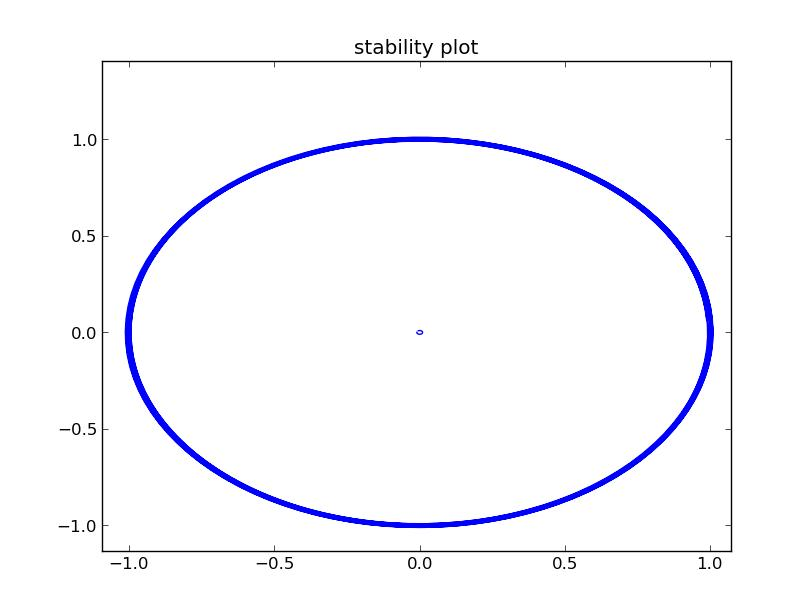
\includegraphics[scale=0.2]{unstable_dt_0,01.jpg}}
  \end{center}
 \caption{\textit{ }}
  \label{fig:edge}
\end{figure}

I found that for most cases dt = 0,01 is fine. you could use bigger dt, possibly  up to dt = 0,05. but i used dt = 0,01 to be sure.
One thing to note is that the system gets more unstable the lower the orbit. So if we were to out in mercury, for example, in the 
system, we would probably need a smaller dt.

We can now test the system a little. By trial and error i found that by giving the Earth (or any object placed at 1 Au from the Sun)
that by giving it an initial velocity of $8.884 AUy^{-1}$ it still has an orbit but at $8.885 AUy^{-1}$ i could no longer get an 
orbit. So the object escaped the solar system.

\begin{figure}[H]
  \begin{center}
    \subfigure[Sun Earth initial v = 8.884 AU/y]{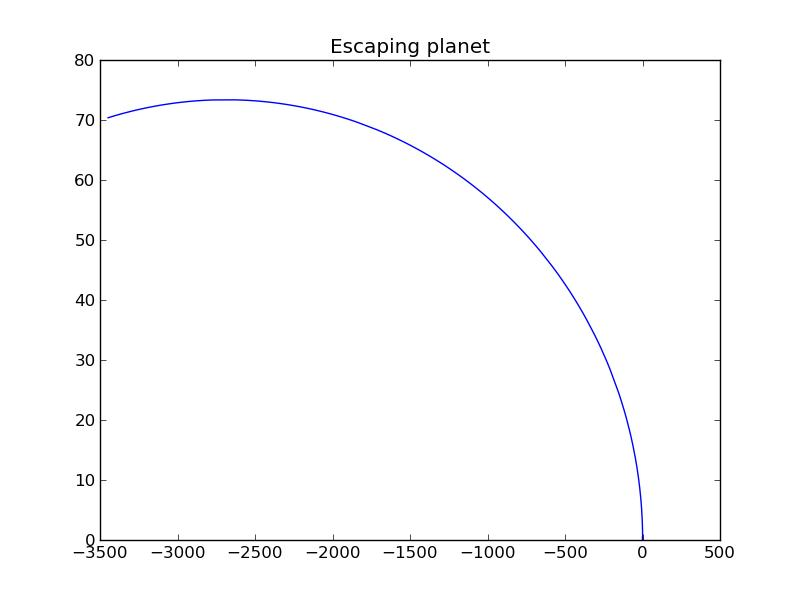
\includegraphics[scale=0.2]{almost_escape.jpg}}
    \subfigure[Sun Earth initial v = 8.885 AU/y]{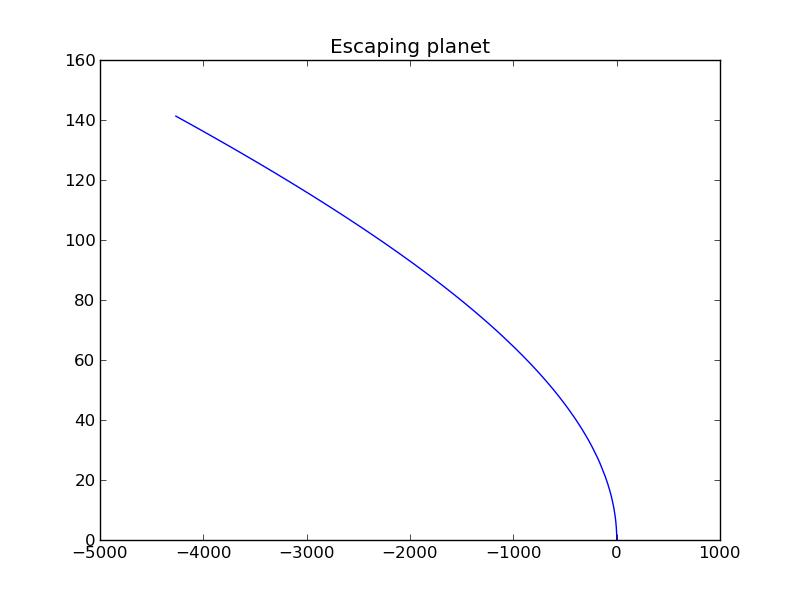
\includegraphics[scale=0.2]{escape.jpg}}
  \end{center}
 \caption{\textit{ }}
  \label{fig:edge}
\end{figure}

This can be explained analytically. From astronomy we know that the total energy in a two body system is given by

\begin{align}
 E = \frac{1}{2} \mu v^2 - \frac{\mu m}{r}, \text{ where } \mu = \frac{m_1 m_2}{m_1 + m_2}, \text{ and } m = G(m_1 + m_2)
\end{align}

In this equation the energy is negative for bound systems, in the case $E = 0$ we get a parabolic trajectory, which means that the 
object will escape. For $E = 0$ we then get

\begin{align}
v = \sqrt{\frac{2 m}{r}} = 8,8848 Auy^{-1}.
\end{align}

This result is very close to what i found by trial and error. We could in fact use this result to find out if any object is bound
to the system or not, and how much increase in velocity it would need to escape.

\begin{figure}[H]
  \begin{center}
    \subfigure[rk4 solver for Jupiter mass with a factor 10]{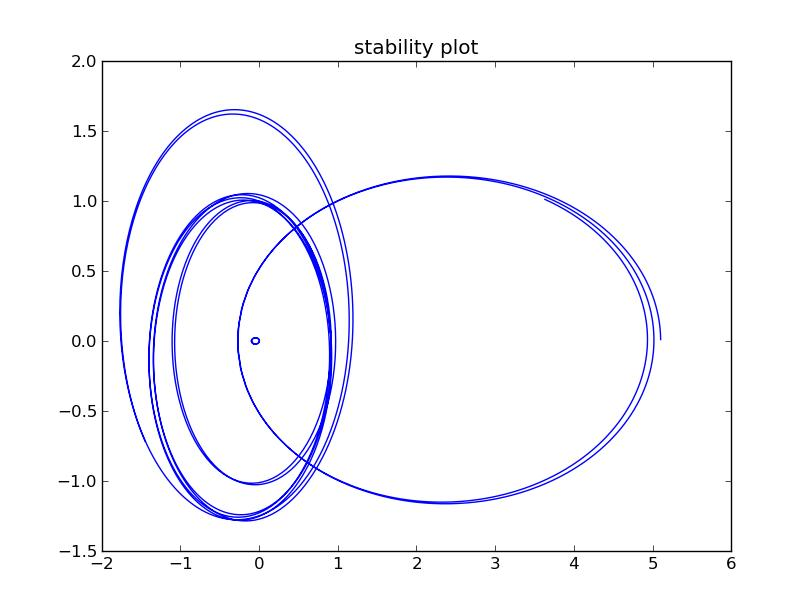
\includegraphics[scale=0.2]{jupiter_m_10_rk4.jpg}}
    \subfigure[rk4 solver for Jupiter mass with a factor 1000]{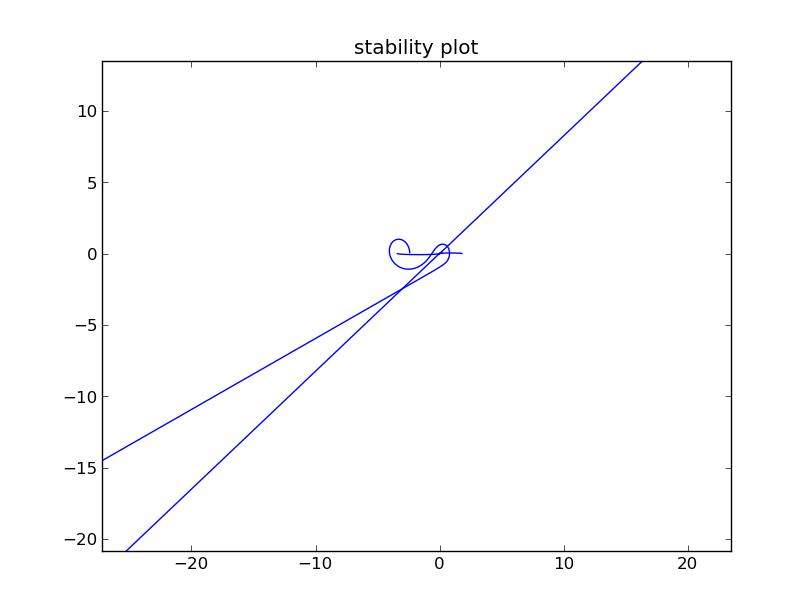
\includegraphics[scale=0.2]{jupiter_m_1000_rk4.jpg}}
    \subfigure[verlet solver for Jupiter mass with a factor 10]{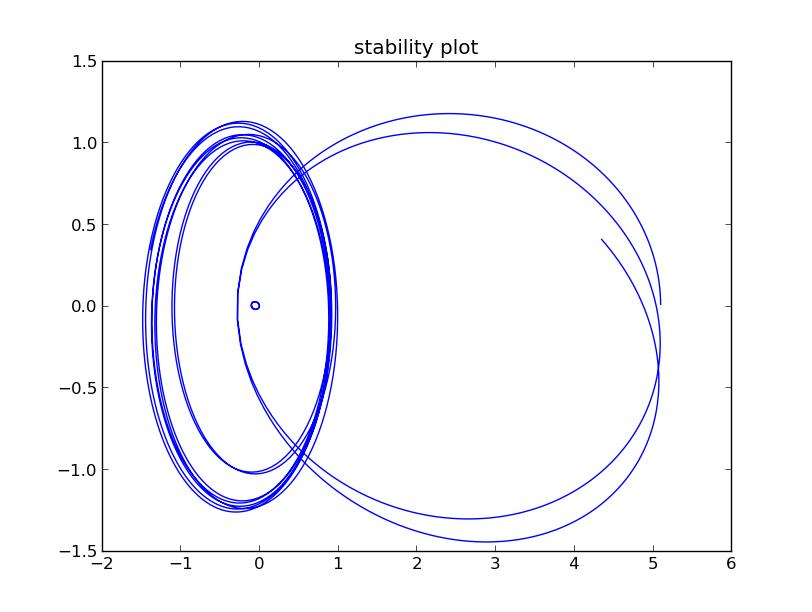
\includegraphics[scale=0.2]{jupiter_m_10_verlet.jpg}}
    \subfigure[verlet solver for Jupiter mass with a factor 1000]{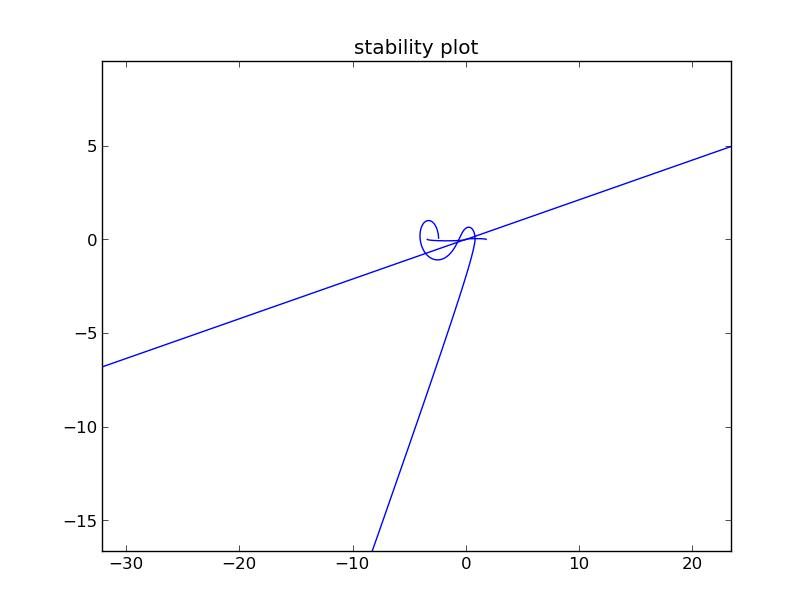
\includegraphics[scale=0.2]{jupiter_m_1000_verlet.jpg}}
    \end{center}
 \caption{\textit{test of solvers with dt = 0,01 }}
  \label{fig:edge}
\end{figure}

In this next plot we test the the different solvers with Jupiter's mass 10 times bigger and 1000 times bigger. We see that the 
solvers seem to be doing almost the same thing. Though, especially for mass = 10 times, we can see that the Verlet solver seems to
be tilting the orbit of Jupiter allot. When i test if the total energy is conserved the Runge Kutta solver keeps the total energy
conserved whilst the Verlet solver seems to be adding energy to the system for each step. I am not sure if this is because the
solver is programmed wrong. But clearly it is not as good as Runge Kutta in my integrator.

\section*{Conclusion}

I have not added all the planets in the system, but in theory this should be easy and it should not alter the results in this 
paper much since the Sun and Jupiter are the dominating objects in our solar system. What could be fun to do would be to add all
the objects in the system, also the moons, and see what happens with the moons of Saturn. It was told in one lecture that 
it is impossible to predict the motion of the moons of Saturn, if this is true then a model should also yield different results 
every time. If not that means that it is not impossible, we just cant accurately determine the initial values, jet.

For future development of the system i would like to implement adaptive Runge Kutta methods. Especially for modeling moons around
planets. In that case you would want a much smaller dt for the moons who have a wery small orbit in contrast to the planets. If
we where to fully model the solar system with this static Runge Kutta algorithm, we would probably lose precision or have a really 
slow code.



%\subsection*{}

%\begin{figure}[H]
%  \begin{center}
%    \subfigure[N = 10]{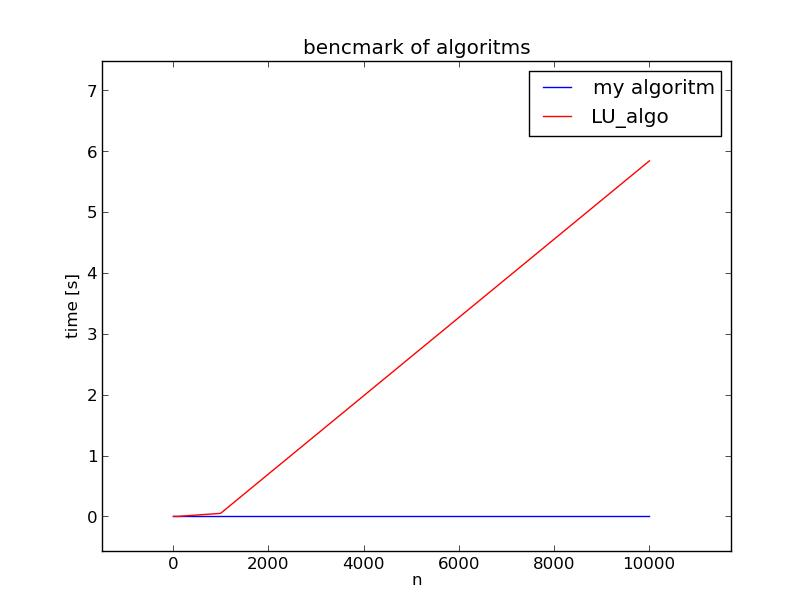
\includegraphics[scale=0.5]{benchmark.jpg}}
%  \end{center}
% \caption{\textit{plot benchmark times for the two different methods of solving}}
%  \label{fig:edge}
%\end{figure}

 
\newpage

\section*{Attachments}

rk4 figure lent from:

$http://www.physics.drexel.edu/students/courses/Comp_Phys/Integrators/rk4.html$

%\textbf{Attachment 1: C++ main program}\newline

%\lstinputlisting[language=C++]{main.cpp}

%\newpage

\end{document}








